\documentclass[tikz]{standalone}

\usepackage{graphicx}
\usepackage{tikz}
\usetikzlibrary{arrows.meta, automata, positioning, quotes}

\tikzstyle{every picture} = [node distance=1.3cm]


\begin{document} 
        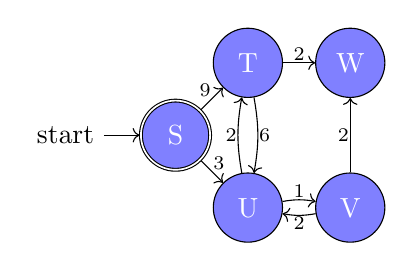
\begin{tikzpicture} [every edge quotes/.append style={font=\scriptsize, inner xsep=.1mm, inner ysep=.2mm}]
            \node (node 1) [circle,text=white,fill=blue!50,initial,state,accepting] {S};
            \node (node 2) [circle,text=white,fill=blue!50,state,above right of= node 1] {T};
            \node (node 3) [circle,text=white,fill=blue!50,state,below right of= node 1] {U};
            \node (node 4) [circle,text=white,fill=blue!50,state,right of= node 3] {V};
            \node (node 5) [circle,text=white,fill=blue!50,state,right of= node 2] {W};
            
            \path (node 1) edge[->,"9",] (node 2)
                  (node 1) edge[->,"3",] (node 3)
                  (node 2) edge[->,"6",bend left=10] (node 3)
                  (node 2) edge[->,"2",] (node 5)
                  (node 3) edge[->,"2",bend left=10] (node 2)
                  (node 3) edge[->,"1",bend left=10] (node 4)
                  (node 4) edge[->,"2",bend left=10] (node 3)
                  (node 4) edge[->,"2",] (node 5);
        \end{tikzpicture}
\end{document}

